\documentclass[12pt]{article}
\usepackage[a4paper,margin=1.25cm]{geometry}
\usepackage{amsmath,amssymb,mathtools}
\usepackage{graphicx}
\usepackage{booktabs}
\usepackage{tabularx}
\usepackage{tikz}
\usepackage[T1]{fontenc}
\usepackage[utf8]{inputenc}
\usepackage[english]{babel}

\setlength{\parindent}{0pt}
\setlength{\parskip}{0.45em}
\setlength{\abovedisplayskip}{5pt plus 1pt minus 1pt}
\setlength{\belowdisplayskip}{5pt plus 1pt minus 1pt}
\setlength{\abovedisplayshortskip}{3pt plus 1pt minus 1pt}
\setlength{\belowdisplayshortskip}{3pt plus 1pt minus 1pt}

\newcommand{\dd}{\,\mathrm{d}}
\newcommand{\e}{\mathrm{e}}
\newcommand{\D}{D}

\begin{document}

\begin{center}
{\Large\bfseries A double integral that is constant on symmetry orbits}\\[0.35em]
{\large two involutions of the disk flatten the integrand to \(\pi/8\)}
\end{center}

\[
\boxed{\displaystyle
\iint_{x^2+y^2\le1}
\frac{\arctan\dfrac{1+x^2}{1+y^2}}{1+\e^{-y}}
\dd x\dd y
=\frac{\pi^2}{8}.}
\]

\textbf{Overview.}
The integrand looks unpleasant: a logistic weight in \(y\) alone,
multiplying an arctangent of a ratio. It is never evaluated. Instead one
observes that the disk carries four measure-preserving maps under which
the integral is invariant, and that the sum of the four transported
copies of the integrand is the constant \(\pi/2\). Averaging, the
integrand may be replaced by \(\pi/8\) without changing the value, and
the answer is \(\pi/8\) times the area of the disk.

Two elementary identities carry the whole argument:
\[
\sigma(t)+\sigma(-t)=1,\qquad \sigma(t)=\frac1{1+\e^{-t}},
\tag{1}
\]
\[
\arctan u+\arctan\frac1u=\frac\pi2,\qquad u>0.
\tag{2}
\]
The first kills the logistic factor, the second kills the arctangent.

\section*{1. Notation and the symmetry group}

Write \(\D=\{(x,y):x^2+y^2\le1\}\) and
\[
A(x,y)=\arctan\frac{1+x^2}{1+y^2},
\qquad
\sigma(t)=\frac1{1+\e^{-t}},
\qquad
g(x,y)=A(x,y)\,\sigma(y),
\]
so that \(I=\iint_\D g\).

Consider the four maps of the plane
\[
T_1(x,y)=(x,y),\quad
T_2(x,y)=(x,-y),\quad
T_3(x,y)=(y,x),\quad
T_4(x,y)=(y,-x).
\tag{3}
\]
Each is linear with determinant \(\pm1\), hence preserves Lebesgue
measure, and each preserves \(x^2+y^2\), hence maps \(\D\) bijectively
onto itself. \(T_2\) is the reflection in the \(x\)-axis, \(T_3\) the
reflection in the diagonal \(y=x\), and \(T_4=T_2T_3\) a quarter turn.

Consequently, for every \(j\),
\[
\iint_\D g(T_j(x,y))\dd x\dd y=\iint_\D g(x,y)\dd x\dd y=I,
\]
and averaging the four identities,
\[
I=\frac14\iint_\D
\Bigl[g(x,y)+g(x,-y)+g(y,x)+g(y,-x)\Bigr]\dd x\dd y.
\tag{4}
\]
No property of \(g\) has been used so far; (4) holds for any integrable
\(g\).

\begin{center}
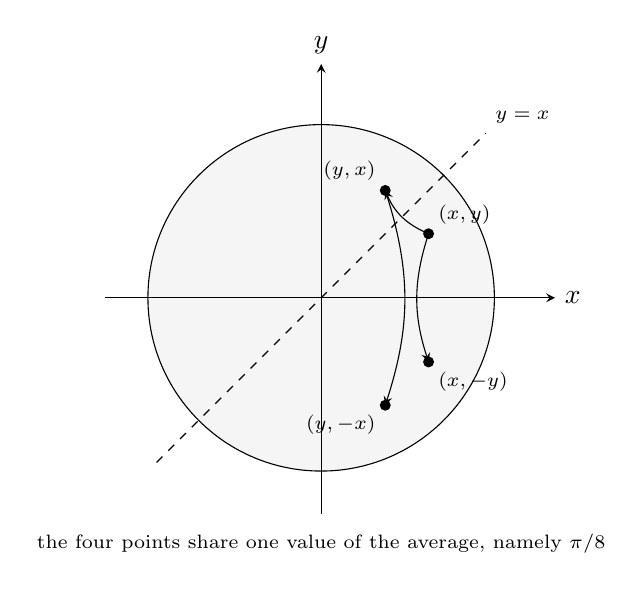
\begin{tikzpicture}[scale=2.2,>=stealth]
\draw[fill=black!4] (0,0) circle (1);
\draw[->] (-1.25,0)--(1.35,0) node[right] {\(x\)};
\draw[->] (0,-1.25)--(0,1.35) node[above] {\(y\)};
\draw[dashed] (-0.95,-0.95)--(0.95,0.95) node[above right] {\scriptsize \(y=x\)};
\coordinate (P) at (0.62,0.37);
\coordinate (P2) at (0.62,-0.37);
\coordinate (P3) at (0.37,0.62);
\coordinate (P4) at (0.37,-0.62);
\fill (P) circle (0.9pt) node[above right] {\scriptsize \((x,y)\)};
\fill (P2) circle (0.9pt) node[below right] {\scriptsize \((x,-y)\)};
\fill (P3) circle (0.9pt) node[above left] {\scriptsize \((y,x)\)};
\fill (P4) circle (0.9pt) node[below left] {\scriptsize \((y,-x)\)};
\draw[->] (P) to[bend right=18] (P2);
\draw[->] (P3) to[bend left=18] (P4);
\draw[->] (P) to[bend left=22] (P3);
\node at (0,-1.42) {\scriptsize the four points share one value of the average, namely \(\pi/8\)};
\end{tikzpicture}
\end{center}

\section*{2. The logistic factor pairs off}

The function \(A\) depends on \(y\) only through \(y^2\), so
\(A(x,-y)=A(x,y)\) and \(A(y,-x)=A(y,x)\). Using (1) twice,
\[
g(x,y)+g(x,-y)
=A(x,y)\bigl[\sigma(y)+\sigma(-y)\bigr]
=A(x,y),
\tag{5}
\]
\[
g(y,x)+g(y,-x)
=A(y,x)\bigl[\sigma(x)+\sigma(-x)\bigr]
=A(y,x).
\tag{6}
\]
The logistic weight has vanished from the problem. Its only relevant
property was
\[
\sigma(t)+\sigma(-t)
=\frac1{1+\e^{-t}}+\frac1{1+\e^{t}}
=\frac{1+\e^{t}+1+\e^{-t}}{(1+\e^{-t})(1+\e^{t})}
=1,
\]
since \((1+\e^{-t})(1+\e^{t})=2+\e^{t}+\e^{-t}\).

\section*{3. The arctangent pairs off}

Put
\[
u=\frac{1+x^2}{1+y^2}>0,
\qquad\text{so that}\qquad
\frac{1+y^2}{1+x^2}=\frac1u .
\]
Then \(A(x,y)=\arctan u\) and \(A(y,x)=\arctan\frac1u\), and (2) gives
\[
A(x,y)+A(y,x)=\frac\pi2.
\tag{7}
\]
Identity (2) itself is immediate: for \(u>0\) the angles
\(\alpha=\arctan u\) and \(\beta=\arctan\frac1u\) are the two acute
angles of the right triangle with legs \(1\) and \(u\), so
\(\alpha+\beta=\pi/2\). Analytically, the derivative of
\(\arctan u+\arctan\frac1u\) is
\(\frac1{1+u^2}-\frac{1/u^2}{1+1/u^2}=0\) on \((0,\infty)\), and the
value at \(u=1\) is \(\frac\pi4+\frac\pi4\).

Adding (5) and (6) and inserting (7),
\[
\boxed{\displaystyle
g(x,y)+g(x,-y)+g(y,x)+g(y,-x)=\frac\pi2
\quad\text{for all }(x,y).}
\tag{8}
\]
This is a pointwise identity, valid on the whole plane, not merely in the
mean.

\section*{4. Conclusion}

Substituting (8) into (4), the bracket is the constant \(\pi/2\), so
\[
I=\frac14\iint_\D\frac\pi2\dd x\dd y
=\frac\pi8\operatorname{area}(\D)
=\frac\pi8\cdot\pi
=\frac{\pi^2}{8}.
\]

The geometric reading is that \(g\) itself is a genuinely lopsided
surface over the disk, larger where \(y>0\) because of the
logistic weight, but the four-point symmetry orbit of any point
carries a fixed total height \(\pi/2\). Integration only sees orbit
averages, and every orbit average equals \(\pi/8\).

\section*{5. What the problem really requires}

Each ingredient can be replaced. Here is exactly what is used.

\begin{center}
\small
\renewcommand{\arraystretch}{1.4}
\begin{tabularx}{\textwidth}{@{}>{\raggedright\arraybackslash}p{0.26\textwidth}X@{}}
\toprule
Ingredient & Property actually used \\
\midrule
The domain \(\D\)
& Invariance under \((x,y)\mapsto(x,-y)\) and \((x,y)\mapsto(y,x)\).
Any such region works: a disk, a square \([-a,a]^2\), an annulus, the
whole plane with an integrable weight. \\
\addlinespace
The weight \(\sigma(y)=(1+\e^{-y})^{-1}\)
& Only \(\sigma(t)+\sigma(-t)=1\). Equivalently
\(\sigma=\frac12+\text{odd}\). Examples:
\(\frac12(1+\tanh y)\), \(\frac12+\frac{\arctan y}{\pi}\),
\(\frac12+y^3\e^{-y^2}\). \\
\addlinespace
The ratio \(\dfrac{1+x^2}{1+y^2}\)
& Only that it is positive, even in each variable separately, and
inverted by the swap \(x\leftrightarrow y\). Examples:
\(\frac{a+x^4}{a+y^4}\), \(\e^{x^2-y^2}\), \(\frac{\cosh x}{\cosh y}\). \\
\addlinespace
\(\arctan\)
& Only the reflection law \(\varphi(u)+\varphi(1/u)=\text{const}\). \\
\bottomrule
\end{tabularx}
\end{center}

This yields the general statement.

\textbf{Proposition.}
Let \(\D\subset\mathbb R^2\) have finite area and be invariant under
\((x,y)\mapsto(x,-y)\) and \((x,y)\mapsto(y,x)\). Let \(h>0\) be even in
each variable separately with \(h(x,y)h(y,x)=1\), and let \(\sigma\)
satisfy \(\sigma(t)+\sigma(-t)=1\). Then
\[
\boxed{\displaystyle
\iint_\D \arctan\bigl(h(x,y)\bigr)\,\sigma(y)\dd x\dd y
=\frac\pi8\operatorname{area}(\D).}
\tag{9}
\]

\textit{Proof.} Identical to Sections 2--4: average over
\(T_1,\dots,T_4\), use \(\sigma(t)+\sigma(-t)=1\) to remove \(\sigma\),
then \(\arctan h+\arctan h^{-1}=\pi/2\). \(\square\)

\section*{6. Why the direct approach fails}

The natural first move, integrating in \(y\) for fixed \(x\) or
passing to polar coordinates, fails: neither the logistic factor nor
the arctangent has an elementary antiderivative in this combination, and
polar coordinates destroy the \(x\leftrightarrow y\) structure by mixing
both variables into \(\theta\). The question to ask is which maps preserve
the domain, and what the integrand does under them. Here the integrand is
not invariant under any single one of those maps, which is why the
symmetrisation (4), an average rather than an identification, is the right
instrument.

Numerically, adaptive quadrature over the disk gives
\(1.2337005\ldots\), against
\(\pi^2/8=1.2337005501\ldots\), consistent to the accuracy of the
quadrature.

\end{document}
